\documentclass[12pt,a4paper]{article}

%% ---------------- Packages ----------------
\usepackage[a4paper,margin=2.5cm]{geometry}
\usepackage[T1]{fontenc}
\usepackage[utf8]{inputenc}
\usepackage{lmodern}
\usepackage{microtype}
\usepackage{amsmath}
\usepackage{graphicx}
\usepackage{xcolor}
\usepackage{booktabs}
\usepackage{array}
\usepackage{tabularx}
\usepackage{longtable}
\usepackage{enumitem}
\usepackage{float}
\usepackage[font=small,labelfont=bf]{caption}
\usepackage{fancyhdr}
\usepackage{titlesec}
\usepackage{tikz}
\usetikzlibrary{arrows.meta,shapes.geometric,calc}
\usepackage[hidelinks]{hyperref}

%% ---------------- Style ----------------
\definecolor{accent}{HTML}{157A5C}
\setlist{nosep,leftmargin=*}
\setlength{\parindent}{0pt}
\setlength{\parskip}{6pt}
\renewcommand{\arraystretch}{1.25}

\titleformat{\section}{\Large\bfseries\color{accent}}{\thesection}{0.6em}{}
\titleformat{\subsection}{\large\bfseries}{\thesubsection}{0.6em}{}
\titleformat{\subsubsection}{\normalsize\bfseries}{\thesubsubsection}{0.6em}{}
\titlespacing*{\section}{0pt}{18pt}{8pt}
\titlespacing*{\subsection}{0pt}{12pt}{6pt}

\pagestyle{fancy}
\fancyhf{}
\lhead{\small UCS503 Software Engineering Lab}
\rhead{\small Personal Finance Manager}
\cfoot{\small\thepage}
\renewcommand{\headrulewidth}{0.4pt}

% TikZ styles shared by all diagrams
\tikzset{
  >={Stealth[length=4pt]},
  flow/.style={->,thick},
  box/.style={draw,rounded corners=2pt,align=center,font=\footnotesize,minimum height=0.8cm,fill=white},
  proc/.style={box,fill=black!8,minimum height=0.9cm},
  store/.style={draw,align=center,font=\footnotesize,minimum height=0.8cm,fill=white},
  lbl/.style={font=\scriptsize,inner sep=1.5pt}
}

% Use-case template table: ID/name, actor+priority, trigger, pre, post, main flow, alternate flows
\newcommand{\usecase}[7]{%
  \begin{table}[H]
  \centering
  \caption{#1}
  \begin{tabularx}{\textwidth}{@{}>{\bfseries}p{3.2cm}X@{}}
    \toprule
    Actor, priority & #2 \\
    Trigger & #3 \\
    Preconditions & #4 \\
    Postconditions & #5 \\
    \midrule
    Main flow & \begin{enumerate}[label=\arabic*.]#6\end{enumerate} \\
    \midrule
    Alternate flows & \begin{itemize}#7\end{itemize} \\
    \bottomrule
  \end{tabularx}
  \end{table}}

\begin{document}

%% ---------------- Title page ----------------
\begin{titlepage}
  \centering
  \vspace*{1.5cm}
  {\large Computer Science and Engineering Department\\[2pt] Thapar Institute of Engineering \& Technology (TIET), Patiala\par}
  \vspace{2cm}
  {\large UCS503 -- Software Engineering Lab\par}
  \vspace{0.6cm}
  {\Huge\bfseries Personal Finance Manager\par}
  \vspace{0.5cm}
  {\Large A Desktop-Based Financial Tracking and Budgeting System\par}
  \vspace{0.8cm}
  {\large UCS 503 Software Engineering Project Report\\[4pt] \textbf{Lab Evaluation}\par}
  \vfill
  \begin{tabular}{@{}p{7cm}p{7cm}@{}}
    \textbf{Submitted by} & \textbf{Submitted to}\\[4pt]
    Arjun Puri (1024030022) & Dr.\ Paramveer Sidhu\\
    Anshdeep Singh (1024030105) & \\
    BE Third Year, COE & \\
  \end{tabular}
  \vspace{2cm}
\end{titlepage}

%% ---------------- Table of contents ----------------
\pagenumbering{roman}
\tableofcontents
\clearpage
\pagenumbering{arabic}

%% =====================================================
\section{Project Selection Phase}

\subsection{Software Bid}
We bid to deliver a lightweight desktop Finance Manager that logs income and expenses, enforces budgets, tracks savings goals and shows the result on a live dashboard.

\textbf{Deliverables.}
\begin{itemize}
  \item \textbf{Application:} modular Python and Tkinter desktop app.
  \item \textbf{Database:} MySQL relational schema with an ER diagram.
  \item \textbf{Documents:} SRS, workflow and analysis diagrams.
  \item \textbf{Testing:} unit tests and a regression checklist.
  \item \textbf{Final demo:} report, presentation and live demonstration.
\end{itemize}

\textbf{Measurable targets.}
\begin{itemize}
  \item Dashboard refresh within 1 second for up to 5,000 transactions.
  \item 100\% match with hand-calculated figures on a fixed test set.
  \item Three-layer, open-source stack that runs on a standard student laptop.
\end{itemize}

\subsection{Project Overview}

\subsubsection{Problem}
Students' money moves through too many places:
\begin{itemize}
  \item \textbf{Fragmentation:} spending is remembered informally or scattered across bank SMS alerts, UPI apps and cash, with no single record.
  \item \textbf{Low visibility:} there is no quick view of actual spending against a monthly budget.
  \item \textbf{No goal tracking:} savings targets, such as a laptop or a trip, have no visible progress measure.
  \item \textbf{Manual entry:} rent, subscriptions and bills are re-entered from memory each month, which invites errors.
\end{itemize}
On a limited, irregular monthly budget, small gains in visibility and habit-tracking can noticeably improve financial discipline and reduce overspending.

\subsubsection{Solution}
The system is a desktop application with five modules.

\begin{table}[H]
\centering
\caption{Application modules}
\begin{tabularx}{\textwidth}{@{}cp{4.3cm}X@{}}
  \toprule
  \textbf{No.} & \textbf{Module} & \textbf{Description}\\
  \midrule
  01 & Transaction entry & Log income and expenses with amount, category, date and description.\\
  02 & Budget engine & Monthly or category limits with the remaining budget in real time.\\
  03 & Savings goals & Target, saved amount, deadline and a visible progress percentage.\\
  04 & Recurring expenses & Rent, subscriptions and bills by frequency; due items are surfaced.\\
  05 & Dashboard and reports & Balance, summaries, and category and monthly charts.\\
  \bottomrule
\end{tabularx}
\end{table}

Every dashboard figure is a deterministic, auditable formula:
\begin{align*}
  \text{Balance} &= \text{Total Income} - \text{Total Expenses}\\
  \text{Savings rate} &= \frac{\text{Savings}}{\text{Income}} \times 100\\
  \text{Budget remaining} &= \text{Limit} - \text{Actual Spending}\\
  \text{Goal progress} &= \frac{\text{Saved}}{\text{Target}} \times 100
\end{align*}

\subsubsection{Architecture}
The application has three layers built on mature open-source engines.

\begin{figure}[H]
\centering
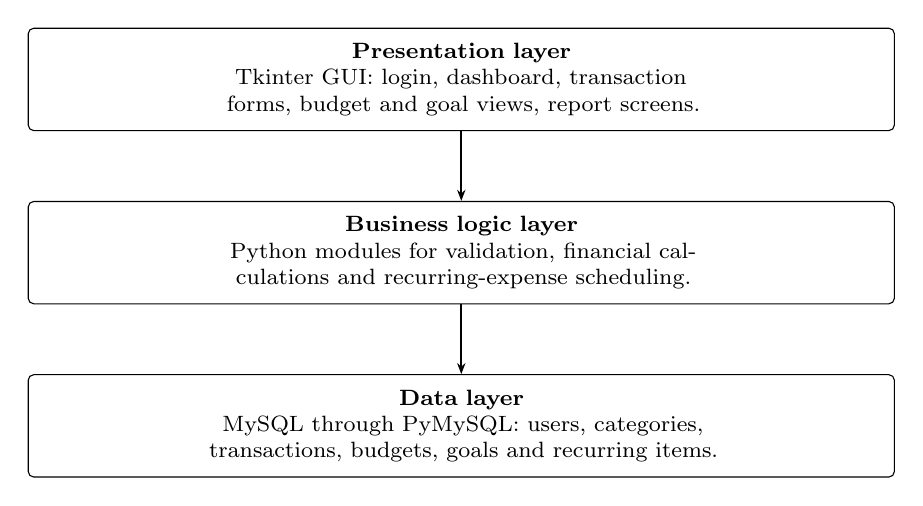
\begin{tikzpicture}
  \node[box,minimum width=11cm,minimum height=1.3cm,text width=10.6cm] (p) at (0,0)
    {\textbf{Presentation layer}\\Tkinter GUI: login, dashboard, transaction forms, budget and goal views, report screens.};
  \node[box,minimum width=11cm,minimum height=1.3cm,text width=10.6cm] (b) at (0,-2.2)
    {\textbf{Business logic layer}\\Python modules for validation, financial calculations and recurring-expense scheduling.};
  \node[box,minimum width=11cm,minimum height=1.3cm,text width=10.6cm] (d) at (0,-4.4)
    {\textbf{Data layer}\\MySQL through PyMySQL: users, categories, transactions, budgets, goals and recurring items.};
  \draw[flow] (p) -- (b);
  \draw[flow] (b) -- (d);
\end{tikzpicture}
\caption{Three-layer architecture}
\end{figure}

\begin{table}[H]
\centering
\caption{Technology stack}
\begin{tabular}{@{}ll@{}}
  \toprule
  \textbf{Engine} & \textbf{Role in the project}\\
  \midrule
  Python & Logic, validation, orchestration\\
  Tkinter & Desktop GUI for all screens\\
  MySQL & Persistent relational database\\
  PyMySQL & Python-to-MySQL connectivity\\
  Matplotlib & Monthly and category charts\\
  datetime & Recurring dates, scheduling\\
  CSV module & Optional transaction export\\
  \bottomrule
\end{tabular}
\end{table}

\subsubsection{Current progress}
\textbf{Built.}
\begin{itemize}
  \item Login screen with MySQL authentication (PyMySQL, parameterised query).
  \item Dashboard shell with sidebar and seven module pages.
  \item Dashboard widgets: summary cards, bar chart, budget bars, recent items, goals, cash-flow donut.
  \item Income form with required-field, amount and date checks.
\end{itemize}
\textbf{Prototype only.}
\begin{itemize}
  \item Dashboard numbers come from sample data until MySQL is connected.
  \item Transactions, Expense, Budget, Goals, Reports and Settings pages are screens without data logic yet.
\end{itemize}
\textbf{Still to do.}
\begin{itemize}
  \item Save and load transactions in MySQL.
  \item Budget and goal calculations on real data.
  \item Password hashing, unit tests, CSV export, recurring items.
\end{itemize}

%% =====================================================
\section{Analysis Phase}

\subsection{Use Cases}

\subsubsection{Use-Case Diagram}
The system has one actor (the student user) and ten use cases.

\begin{figure}[H]
\centering
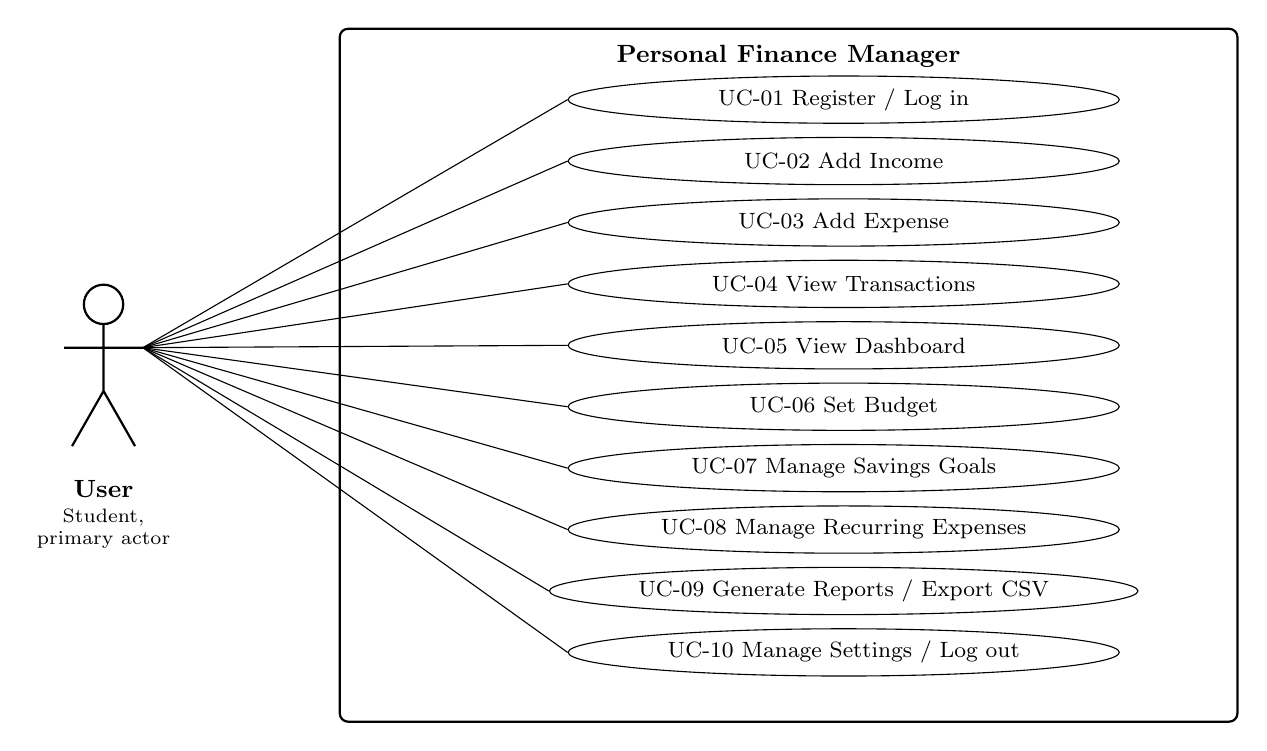
\begin{tikzpicture}[x=1cm,y=1cm]
  % system boundary
  \draw[rounded corners=3pt,thick] (4.2,-0.4) rectangle (15.6,8.4);
  \node[font=\small\bfseries] at (9.9,8.05) {Personal Finance Manager};
  % actor (stick figure)
  \draw[thick] (1.2,4.9) circle (0.25);
  \draw[thick] (1.2,4.65)--(1.2,3.8) (0.7,4.35)--(1.7,4.35) (1.2,3.8)--(0.8,3.1) (1.2,3.8)--(1.6,3.1);
  \node[font=\small\bfseries,align=center] at (1.2,2.55) {User};
  \node[font=\scriptsize,align=center] at (1.2,2.05) {Student,\\primary actor};
  \coordinate (actor) at (1.7,4.35);
  \foreach \i/\txt in {0/{UC-01 Register / Log in},1/{UC-02 Add Income},2/{UC-03 Add Expense},
      3/{UC-04 View Transactions},4/{UC-05 View Dashboard},5/{UC-06 Set Budget},
      6/{UC-07 Manage Savings Goals},7/{UC-08 Manage Recurring Expenses},
      8/{UC-09 Generate Reports / Export CSV},9/{UC-10 Manage Settings / Log out}} {
    \pgfmathsetmacro{\yy}{7.5-0.78*\i}
    \node[draw,ellipse,minimum width=7cm,minimum height=0.6cm,font=\footnotesize,inner sep=1pt] (uc\i) at (10.6,\yy) {\txt};
    \draw (actor) -- (uc\i.west);
  }
\end{tikzpicture}
\caption{Use-case diagram}
\end{figure}

\textbf{Reading the diagram.}
\begin{itemize}
  \item Every use case starts from a successful log in (UC-01).
  \item UC-02 and UC-03 both update the balance shown in UC-05.
  \item UC-09 can export the report as a CSV file.
  \item All data is read from and written to MySQL, scoped to the logged-in user.
\end{itemize}

\subsubsection{Use Case Templates}

\usecase{UC-01 Register / Log in}
  {User (student), High}
  {User opens the application.}
  {MySQL server is running and the user account exists.}
  {A session starts and the dashboard opens, scoped to that user.}
  {\item User enters username and password.
   \item System checks that both fields are filled.
   \item System looks the user up in MySQL.
   \item On a match, the login window hides and the dashboard opens.}
  {\item A field is empty: ``Please enter both username and password.''
   \item No match: ``Invalid username or password.''
   \item Database unreachable: error dialog, user stays on login.}

\usecase{UC-02 Add Income (UC-03 Add Expense follows the same flow)}
  {User (student), High}
  {User opens the Income page and saves a new entry.}
  {User is logged in (UC-01).}
  {Income is saved, the form clears, and balance and totals are recalculated.}
  {\item User enters amount, category, description, date and source.
   \item System checks that no field is empty.
   \item System checks the amount is a number above 0.
   \item System checks the date is valid (DD-MM-YYYY).
   \item System saves the record and confirms it to the user.}
  {\item Missing field: ``Missing Information'' warning.
   \item Amount zero, negative or not a number: ``Invalid Amount''.
   \item Bad date: ``Invalid Date''. Nothing is saved.}

\usecase{UC-06 Set Budget}
  {User (student), High}
  {User clicks ``+ Add Budget'' on the Budget page.}
  {User is logged in and at least one category exists.}
  {Limit is saved; remaining budget updates as expenses are added.}
  {\item User picks a category and a monthly period.
   \item User enters the spending limit.
   \item System checks the limit is above 0 and no budget exists for that category and month.
   \item System saves the budget.
   \item System shows Budget Remaining $=$ Limit $-$ Actual Spending as a progress bar.}
  {\item Invalid limit: error shown, nothing saved.
   \item Budget exists: user is offered an update.
   \item Spending exceeds the limit: over-budget warning.}

\subsection{Activity and Swimlane Diagram}
Figure~\ref{fig:swim} shows the Add Transaction activity across the User, System and MySQL.

\begin{figure}[H]
\centering
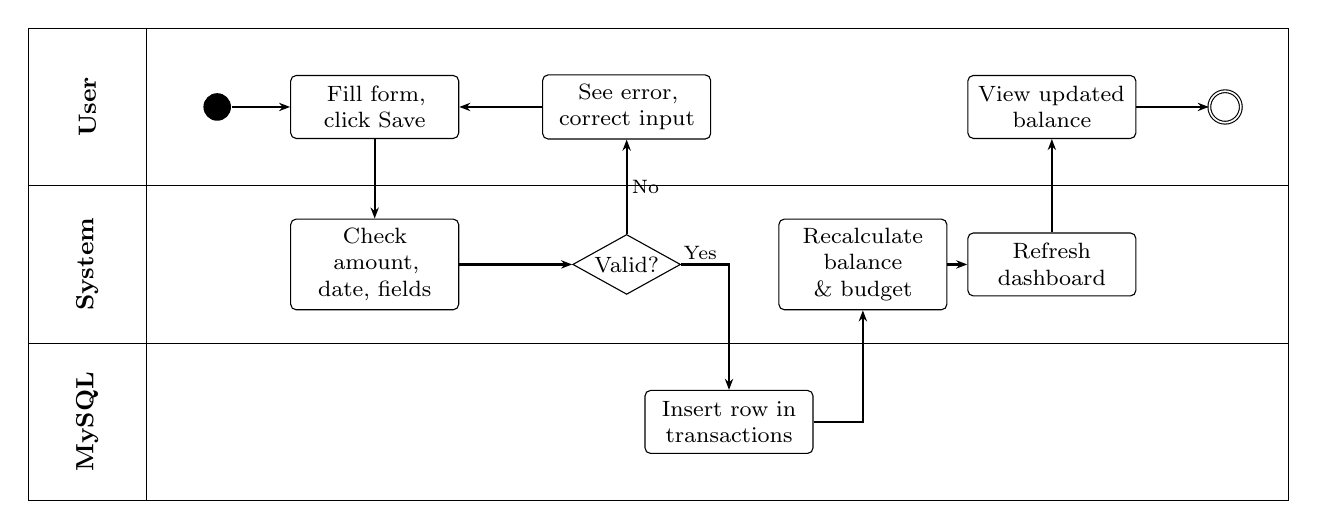
\begin{tikzpicture}[x=1cm,y=1cm,
    nb/.style={box,minimum width=2.1cm,text width=1.9cm}]
  % lanes
  \draw (0,0) rectangle (16,6);
  \draw (0,2) -- (16,2);
  \draw (0,4) -- (16,4);
  \draw (1.5,0) -- (1.5,6);
  \node[font=\small\bfseries,rotate=90] at (0.75,5) {User};
  \node[font=\small\bfseries,rotate=90] at (0.75,3) {System};
  \node[font=\small\bfseries,rotate=90] at (0.75,1) {MySQL};
  % nodes
  \node[circle,fill=black,minimum size=0.35cm,inner sep=0] (start) at (2.4,5) {};
  \node[nb] (fill) at (4.4,5) {Fill form,\\click Save};
  \node[nb] (err) at (7.6,5) {See error,\\correct input};
  \node[nb] (view) at (13.0,5) {View updated\\balance};
  \node[circle,draw,double,minimum size=0.4cm,inner sep=0] (end) at (15.2,5) {};
  \node[nb] (check) at (4.4,3) {Check amount,\\date, fields};
  \node[diamond,draw,aspect=1.8,inner sep=1pt,font=\footnotesize] (valid) at (7.6,3) {Valid?};
  \node[nb] (recalc) at (10.6,3) {Recalculate\\balance \& budget};
  \node[nb] (refresh) at (13.0,3) {Refresh\\dashboard};
  \node[nb] (ins) at (8.9,1) {Insert row in\\transactions};
  % edges
  \draw[flow] (start) -- (fill);
  \draw[flow] (fill) -- (check);
  \draw[flow] (check) -- (valid);
  \draw[flow] (valid) -- node[lbl,right]{No} (err);
  \draw[flow] (err) -- (fill);
  \draw[flow] (valid.east) -| node[lbl,pos=0.2,above]{Yes} (ins.north);
  \draw[flow] (ins.east) -| (recalc.south);
  \draw[flow] (recalc) -- (refresh);
  \draw[flow] (refresh) -- (view);
  \draw[flow] (view) -- (end);
\end{tikzpicture}
\caption{Activity diagram with swimlanes: Add Transaction}
\label{fig:swim}
\end{figure}

\subsection{Data Flow Diagrams}

\subsubsection{DFD Level 0}
The context diagram shows the system as a single process.

\begin{figure}[H]
\centering
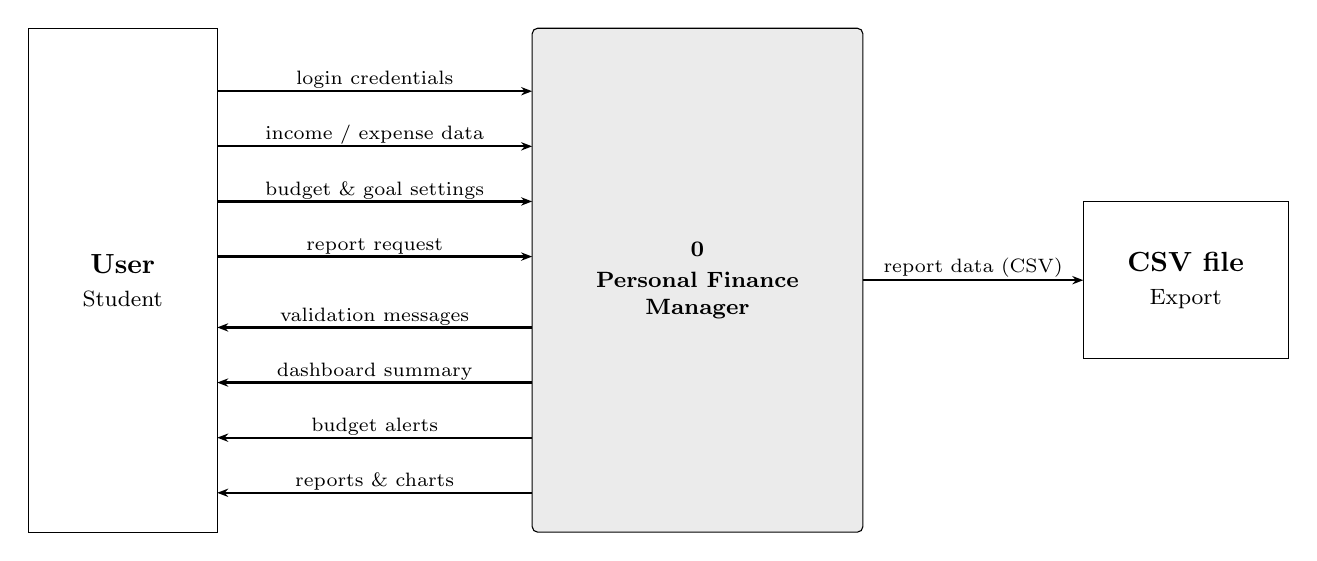
\begin{tikzpicture}[x=1cm,y=1cm]
  \node[draw,minimum width=2.4cm,minimum height=6.4cm,align=center] (user) at (1.2,0) {\textbf{User}\\{\footnotesize Student}};
  \node[proc,minimum width=4.2cm,minimum height=6.4cm,fill=black!8] (sys) at (8.5,0) {\textbf{0}\\[2pt]\textbf{Personal Finance}\\\textbf{Manager}};
  \node[draw,minimum width=2.6cm,minimum height=2cm,align=center] (csv) at (14.7,0) {\textbf{CSV file}\\{\footnotesize Export}};
  \foreach \y/\txt in {2.4/{login credentials},1.7/{income / expense data},1.0/{budget \& goal settings},0.3/{report request}}
    \draw[flow] (2.4,\y) -- (6.4,\y) node[midway,above=-1pt,lbl]{\txt};
  \foreach \y/\txt in {-0.6/{validation messages},-1.3/{dashboard summary},-2.0/{budget alerts},-2.7/{reports \& charts}}
    \draw[flow] (6.4,\y) -- (2.4,\y) node[midway,above=-1pt,lbl]{\txt};
  \draw[flow] (10.6,0) -- (13.4,0) node[midway,above=-1pt,lbl]{report data (CSV)};
\end{tikzpicture}
\caption{DFD Level 0 (context diagram)}
\end{figure}

\subsubsection{DFD Level 1}
Level 1 has five processes and four data stores.

\begin{figure}[H]
\centering
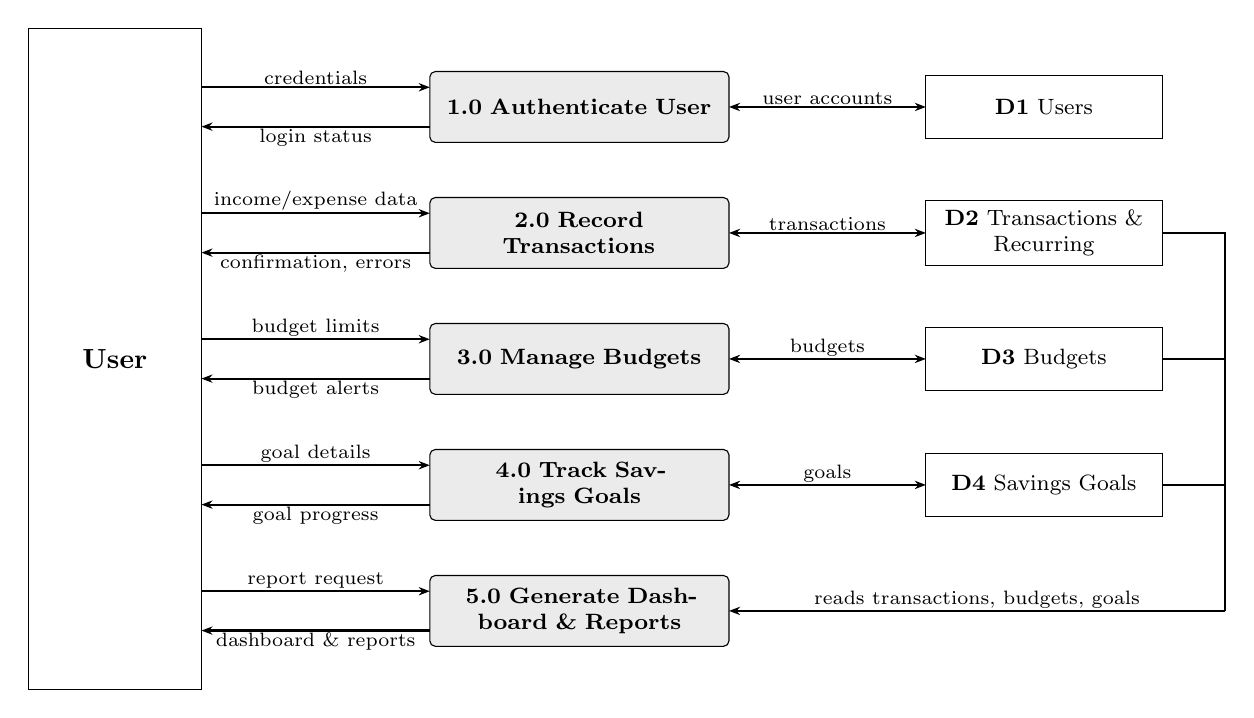
\begin{tikzpicture}[x=1cm,y=1cm,
    bi/.style={<->,thick}]
  \node[draw,minimum width=2.2cm,minimum height=8.4cm] at (1.1,0) {\textbf{User}};
  \foreach \y/\pname/\ina/\outb in {3.2/{1.0 Authenticate User}/{credentials}/{login status},
      1.6/{2.0 Record Transactions}/{income/expense data}/{confirmation, errors},
      0/{3.0 Manage Budgets}/{budget limits}/{budget alerts},
      -1.6/{4.0 Track Savings Goals}/{goal details}/{goal progress},
      -3.2/{5.0 Generate Dashboard \& Reports}/{report request}/{dashboard \& reports}} {
    \node[proc,minimum width=3.8cm,text width=3.5cm] (p\y) at (7,\y) {\textbf{\pname}};
    \draw[flow] (2.2,\y+0.25) -- (5.1,\y+0.25) node[midway,above=-1pt,lbl]{\ina};
    \draw[flow] (5.1,\y-0.25) -- (2.2,\y-0.25) node[midway,below=-1pt,lbl]{\outb};
  }
  \node[store,minimum width=3cm] at (12.9,3.2) {\textbf{D1} Users};
  \node[store,minimum width=3cm] at (12.9,1.6) {\textbf{D2} Transactions \&\\Recurring};
  \node[store,minimum width=3cm] at (12.9,0) {\textbf{D3} Budgets};
  \node[store,minimum width=3cm] at (12.9,-1.6) {\textbf{D4} Savings Goals};
  \draw[bi] (8.9,3.2) -- (11.4,3.2) node[midway,above=-1pt,lbl]{user accounts};
  \draw[bi] (8.9,1.6) -- (11.4,1.6) node[midway,above=-1pt,lbl]{transactions};
  \draw[bi] (8.9,0) -- (11.4,0) node[midway,above=-1pt,lbl]{budgets};
  \draw[bi] (8.9,-1.6) -- (11.4,-1.6) node[midway,above=-1pt,lbl]{goals};
  % read bus for process 5.0
  \draw[thick] (14.4,1.6) -- (15.2,1.6) -- (15.2,-3.2);
  \draw[thick] (14.4,0) -- (15.2,0);
  \draw[thick] (14.4,-1.6) -- (15.2,-1.6);
  \draw[flow] (15.2,-3.2) -- (8.9,-3.2) node[midway,above=-1pt,lbl]{reads transactions, budgets, goals};
\end{tikzpicture}
\caption{DFD Level 1}
\end{figure}

\subsubsection{DFD Level 2}
Process 2.0 (Record Transactions) expanded. Budget usage and goal progress are derived in Processes 3.0, 4.0 and 5.0 (Level 1).

\begin{figure}[H]
\centering
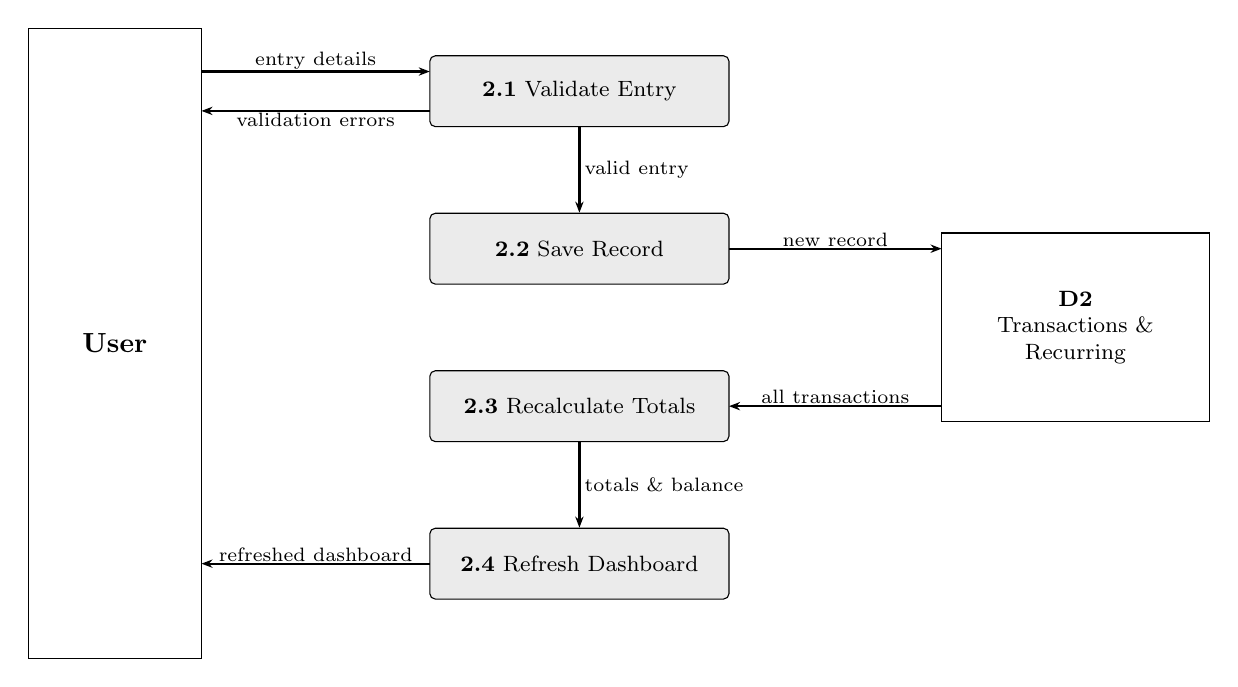
\begin{tikzpicture}[x=1cm,y=1cm]
  \node[draw,minimum width=2.2cm,minimum height=8cm] at (1.1,0) {\textbf{User}};
  \node[proc,minimum width=3.8cm] (v) at (7,3.2)  {\textbf{2.1} Validate Entry};
  \node[proc,minimum width=3.8cm] (s) at (7,1.2)  {\textbf{2.2} Save Record};
  \node[proc,minimum width=3.8cm] (r) at (7,-0.8) {\textbf{2.3} Recalculate Totals};
  \node[proc,minimum width=3.8cm] (f) at (7,-2.8) {\textbf{2.4} Refresh Dashboard};
  \node[store,minimum width=3.4cm,minimum height=2.4cm] at (13.3,0.2) {\textbf{D2}\\Transactions \&\\Recurring};
  \draw[flow] (2.2,3.45) -- (5.1,3.45) node[midway,above=-1pt,lbl]{entry details};
  \draw[flow] (5.1,2.95) -- (2.2,2.95) node[midway,below=-1pt,lbl]{validation errors};
  \draw[flow] (v) -- (s) node[midway,right,lbl]{valid entry};
  \draw[flow] (8.9,1.2) -- (11.6,1.2) node[midway,above=-1pt,lbl]{new record};
  \draw[flow] (11.6,-0.8) -- (8.9,-0.8) node[midway,above=-1pt,lbl]{all transactions};
  \draw[flow] (r) -- (f) node[midway,right,lbl]{totals \& balance};
  \draw[flow] (5.1,-2.8) -- (2.2,-2.8) node[midway,above=-1pt,lbl]{refreshed dashboard};
\end{tikzpicture}
\caption{DFD Level 2: Process 2.0 Record Transactions}
\end{figure}

\subsection{SRS in IEEE Format}

\subsubsection{Introduction}
\textbf{Purpose.} Define the requirements for the Personal Finance Manager desktop application.

\textbf{Scope.} Track income, expenses, budgets, savings goals and recurring items; show a dashboard and reports. Single user per session, local MySQL.

\textbf{Definitions.} DRL: Dashboard Refresh Latency. SRS: Software Requirements Specification. GUI: graphical user interface.

\textbf{References.} IEEE Std 830-1998; project proposal dated 15 August 2026.

\subsubsection{Overall description}
\begin{description}[style=nextline]
  \item[Product perspective] Standalone three-layer desktop app with a MySQL back end.
  \item[Product functions] Transactions, budgets, savings goals, recurring expenses, dashboard and reports.
  \item[Users] Students and individuals with basic computer skills and no accounting background.
  \item[Constraints] Runs on a student laptop; Python, Tkinter and MySQL; no advanced algorithms.
  \item[Assumptions] Python 3 and a local MySQL server are installed and running.
\end{description}

\subsubsection{Functional requirements}
\begin{table}[H]
\centering
\caption{Functional requirements (the system shall\ldots)}
\begin{tabularx}{\textwidth}{@{}lXll@{}}
  \toprule
  \textbf{ID} & \textbf{Requirement} & \textbf{Priority} & \textbf{Status}\\
  \midrule
  FR-01 & register users and authenticate them by username and password & High & Login built\\
  FR-02 & record income: amount, category, date, description, source & High & Form built\\
  FR-03 & record expenses: amount, category, date, description & High & Planned\\
  FR-04 & validate required fields, amount above 0 and valid dates & High & Income only\\
  FR-05 & list the user's transactions with category and date & Medium & Planned\\
  FR-06 & compute balance, savings and savings rate from stored data & High & Sample data\\
  FR-07 & store budgets and show the remaining budget & High & Planned\\
  FR-08 & track savings goals with a progress percentage & Medium & Planned\\
  FR-09 & schedule recurring expenses and surface due items & Medium & Planned\\
  FR-10 & show category and monthly charts; export reports to CSV & Medium & Sample data\\
  FR-11 & restrict every query to the logged-in user's data & High & Planned\\
  \bottomrule
\end{tabularx}
\end{table}

\subsubsection{Non-functional requirements}
\begin{description}[style=nextline]
  \item[NFR-01 Performance] Dashboard refresh within 1 second for up to 5,000 transactions.
  \item[NFR-02 Accuracy] Figures match hand-calculated values on a fixed test dataset.
  \item[NFR-03 Reliability] Measured as the share of test sessions without an unhandled exception.
  \item[NFR-04 Usability] A first-time user adds a transaction and finds the new balance unaided.
  \item[NFR-05 Security] Passwords are hashed; every query is scoped by user.
\end{description}

\subsubsection{External interfaces}
\begin{description}[style=nextline]
  \item[User interface] Tkinter windows: a login screen and a maximised dashboard with sidebar navigation.
  \item[Software interfaces] MySQL through PyMySQL; tkcalendar date picker; Matplotlib charts; CSV export.
  \item[Hardware] A standard student laptop.
  \item[Portability] Layers stay separate so the UI can later move behind a Flask API.
\end{description}

\subsection{User Stories and Story Cards}

\subsubsection{User stories}
\begin{table}[H]
\centering
\caption{User stories}
\begin{tabularx}{\textwidth}{@{}llX@{}}
  \toprule
  \textbf{ID} & \textbf{Priority} & \textbf{Story}\\
  \midrule
  US-01 & High & As a user, I want to log in with my username and password, so that my financial data stays private.\\
  US-02 & High & As a student, I want to record my income with its source and date, so that I know how much money I receive.\\
  US-03 & High & As a student, I want to record each expense by category, so that I can see where my money goes.\\
  US-04 & High & As a user, I want my balance on a dashboard, so that I know where I stand at a glance.\\
  US-05 & High & As a student, I want to set a monthly budget per category, so that I can control my spending.\\
  US-06 & Medium & As a user, I want to see how much budget remains, so that I stop before I overspend.\\
  US-07 & Medium & As a saver, I want a goal with a target and deadline, so that I can watch my progress.\\
  US-08 & Medium & As a user, I want recurring bills tracked automatically, so that I do not re-enter rent and subscriptions each month.\\
  \bottomrule
\end{tabularx}
\end{table}

\subsubsection{Story cards}
\newcommand{\storycard}[4]{%
  \begin{table}[H]
  \centering
  \caption{#1}
  \begin{tabularx}{\textwidth}{@{}>{\bfseries}p{3.2cm}X@{}}
    \toprule
    Story & #2 \\
    Priority & #3 \\
    \midrule
    Acceptance criteria & \begin{itemize}#4\end{itemize} \\
    \bottomrule
  \end{tabularx}
  \end{table}}

\storycard{US-02 Add income}
  {As a student, I want to record my income with its source and date.}
  {High}
  {\item All five fields are required.
   \item Amount is a number above 0.
   \item Date is in DD-MM-YYYY format.
   \item Balance updates on the dashboard within 1 second of saving.}

\storycard{US-05 Set budget}
  {As a student, I want to set a monthly budget per category.}
  {High}
  {\item Limit is a number above 0.
   \item One budget per category per month.
   \item Remaining $=$ Limit $-$ Actual Spending, shown after each expense.
   \item A warning appears when spending passes the limit.}

\storycard{US-08 Recurring items}
  {As a user, I want recurring bills tracked automatically.}
  {Medium}
  {\item Each item stores amount, category, frequency and next due date.
   \item Due items are surfaced automatically.
   \item Resulting transactions appear in history like manual ones.}

%% =====================================================
\section{Next Steps}
From analysis to a working system:
\begin{enumerate}[label=\arabic*.]
  \item Connect every module to MySQL and replace the sample data.
  \item Build budget, goal and balance calculations with unit tests.
  \item Hash passwords and scope every query to the logged-in user.
  \item Measure refresh latency and run the peer pilot.
\end{enumerate}

\end{document}